\documentclass[a4paper, 11pt, final, garamond]{book}
\usepackage{cours-preambule}

\raggedbottom

\makeatletter
\renewcommand{\@chapapp}{Travaux pratiques -- TP}
\makeatother

\let\SavedIndent\indent
\protected\def\indent{%
  \begingroup
    \parindent=\the\parindent
    \SavedIndent
  \endgroup
}
\setlength{\parindent}{0pt}

\begin{document}
\setcounter{chapter}{8}

\chapter{Dosage par \'etalonnage~: spectrophotom\'etrie et conductim\'etrie}

\section{Objectifs}

\begin{itemize}
    \item Revoir le protocole de dilution (niveau lycée).
    \item Revoir la technique de spectrophotométrie.
    \item Vérifier la loi de Beer-Lambert.
    \item Revoir le protocole expérimental de conductimétrie~;
    \item Vérifier la loi de Kohlrausch.
\end{itemize}

\section{S'approprier}

\subsection{Le dosage par étalonnage}

Un dosage par étalonnage consiste à déterminer la concentration molaire d'une
espèce chimique en solution en comparant une grandeur physique (conductance,
absorbance…) de la solution avec la même grandeur physique mesurée pour des
solutions étalons (solution dont on connait avec précision la composition). En
supposant qu'il existe une relation entre la valeur de la grandeur physique et
la concentration, on peut alors déterminer la concentration en une espèce
chimique donnée dans la solution inconnue en comparant la valeur de la grandeur
physique pour cette solution avec la valeur de la grandeur physique pour la
solution étalon.

\subsection{Le principe de la spectrophotométrie}

Certaines espèces chimiques sont capables d'absorber la lumière UV ou visible.
Ainsi, est-il possible de relier l'intensité lumineuse transmise à une longueur
d'onde donnée à la concentration d'une espèce en solution par la \textbf{loi de
Beer-Lambert}~:
\begin{rprop}{Loi de \textsc{Beer-Lambert}}
    \[\boxed{A = \log\left(\frac{I_0}{I}\right) = \sum_{i=1}^{N}\epsilon_i \,
    \ell \, c_i}\]
    Avec~:
    \begin{itemize}
        \item $A$ est l'absorbance (adimensionnée). C'est une grandeur
            \textbf{additive}
        \item $I_0$ l'intensité lumineuse incidente (en $\si{W.m^{-2}}$)
        \item $I$ l'intensité lumineuse en sortie de cuve (en $\si{W.m^{-2}}$)
        \item $\epsilon_i$ le coefficient d'extinction molaire de l'espèce ${\rm
            X}_i$ à la longueur d'onde $\lambda$ (dépend de l'espèce chimique
            étudiée mais aussi marginalement du solvant et de la température)
        \item $\ell$ la largeur de la cuve traversée par le faisceau (en $\si{m}$)
        \item $c$ la concentration en l'espèce absorbante ${\rm X}_i$ (en
            $\si{mol.L^{-1}}$)
    \end{itemize}
\end{rprop}

Ici, on se limite à une unique espèce absorbante, tel que la relation de
Beer-Lambert devient
\[\boxed{A = \log\left(\frac{I_0}{I}\right) = \epsilon \, \ell \, c}\]

La valeur de $\epsilon \, \ell$ est bien souvent inconnue. Pour
obtenir $c_0$ connaissant $A_0$ de notre solution inconnue, il est donc
nécessaire de déterminer préalablement l'expression de la fonction $A=f(c)$.
Cette courbe est appelée \textbf{courbe d'étalonnage}. Elle est obtenue avec
l'ensemble des points de coordonnées $(A_i, c_i)$ obtenus à partir d'un ensemble
de solutions étalons $S_i$ de concentrations connues.

\subsection{Le principe de la conductimétrie}

Cette méthode repose sur l'existence d'ions en solution et sur leur capacité à
faciliter le passage d'un courant. La nature des ions et leurs concentrations
modifient la conductance $G$ du système (grandeur qui est l'inverse de la
résistance $R$) exprimée en \si{S} (Siemens). Plus le milieu est propice au
passage du courant, plus la conductance est élevée. Celle-ci est reliée à trois
paramètres principaux~:

\begin{enumerate}
    \item la conductivité $\sigma$ du système
    \item la longueur $\ell$
    \item la section $S$ de la cellule
\end{enumerate}

La conductance s'exprime alors selon
\[\DS G = \frac{\sigma S}{\ell}\]

Ainsi, on ne parle pas de conductance \cancel{de la solution}, puisque la
conductance dépend de la cellule de mesure et de sa géométrie. L'unité de
conductivité est le $\si{S.m^{-1}}$~; le quotient $K = \ell / S$ est appelé
constante de cellule. Ainsi, on a $G = \sigma / K$. La mesure de la conductance
s'effectue avec un conductimètre, qui est en fait un ohmmètre.\bigbreak

La conductivité $\sigma$ de la solution peut alors s'exprimer par la \textbf{loi
de Kohlrausch}, exprimée sous une forme avec la charge de l'ion~:
\begin{rprop}{Loi de \textsc{Kohlrausch}}
    \[\boxed{\sigma = \sum_{i} \lambda_i \left|z_i\right| [{\rm X}_i]}\]

    Avec~:
    \begin{itemize}
        \item $\lambda_i$ la conductivité molaire ionique de l'ion ${\rm X}_i$ (en
            $\si{S.m^2.mol^{-1}}$) donnée dans les tables
        \item $z_i$ la charge de l'ion ${\rm X}_i$
        \item $[{\rm X}]_i$ la concentration de l'ion ${\rm X}_i$
    \end{itemize}
\end{rprop}

\begin{rror}{Important}
    \begin{center}
        \bfseries
        La conductivité $\sigma$ de la solution prend en compte tous les ions
        présents dans la solution. Il faut donc faire l'inventaire des ions en
        solution avec soin.
    \end{center}
\end{rror}

En supposant que l'on ne fait varier que d'une unique espèce ionique (et donc
conductrice) dans la solution, on pourra noter $c = [{\rm X}_i]$ la concentration de cette espèce.
La \textbf{courbe d'étalonnage} est alors la représentation graphique de $\sigma = f(c)$ obtenue avec l'ensemble des points de coordonnées $(c_i~; \sigma_i)$ où $\sigma_i$ sont les conductivités des différentes solutions étalons $S_i$ de concentration $c_i$. Connaissant la conductivité $\sigma_0$ de la solution $S_0$ inconnue, on en déduit grâce à la courbe d'étalonnage la concentration molaire $c_0$ de la solution $S_0$.


\subsection{Le principe de la dilution}

\begin{rprop}{Dilution}
    On peut diminuer la concentration $c$ d'une solution de volume $V$ en
    ajoutant du solvant jusqu'à un volume $V'$. La concentration $c'$
    obtenue est alors
    \[\boxed{cV = c'V'}
      \Longleftrightarrow
      \boxed{\frac{c}{c'} = \frac{V'}{V}}
  \]
\end{rprop}

En effet, la quantité de matière de soluté ne change pas avec l'ajout de
solvant, autrement dit $n$ est constant. On a donc
\[ c = \frac{n}{V} \qqet c' = \frac{n}{V'}\]
d'où le résultat.

\section{Analyser}

\subsection{Préliminaire sur la solution de permanganate de potassium}

Le permanganate de potassium solide $\ce{KMNO4\sol{}}$, est un antiseptique utilisé pour désinfecter des plaies, les fruits ou
légumes, traiter les eaux… Il se vend en pharmacie sous forme de sachet~: la
notice indique que le sachet contient $\SI{0.25}{g}$ de $\ce{KMNO4\sol{}}$ à
dissoudre dans $\SI{2.5}{L}$ d'eau. C'est ainsi qu'une solution aqueuse $S_0$ de permanganate de
potassium $\ce{K\plus{}\aqu{} + MNO4\moin{}\aqu{}}$ a été obtenue.
Il s'agit ici de vérifier, par deux méthodes différentes, l'indication de masse portée sur le sachet.

\medskip
\begin{rdefi}{\tiny Donnée}
    Masse molaire du permanganate de potassium~: $M = \SI{158,0}{g.mol^{-1}}$.
\end{rdefi}

\begin{minipage}{0.45\linewidth}
    \begin{rexem}{Questions}
        Pourquoi peut-on suivre le dosage du permanganate par
        spectrophotométrie~? Sur l'étiquette du permanganate de potassium, on
        peut voir ces pictogrammes~: que signifient-ils~? quelles précautions
        faut-il prendre~?
    \end{rexem}
\end{minipage}
\begin{minipage}{0.55\linewidth}
    \begin{center}
        
\includegraphics[width=\linewidth]{picto3}
    \end{center}
\end{minipage}

\subsection{Préparation des solutions aqueuses étalon}

On dispose d'une solution-mère aqueuse $S_1$ de permanganate de potassium de concentration molaire
$c_1 = \SI{1.00e-3}{mol.L^{-1}}$. On veut préparer, à partir de cette solution
$S_1$, par dilution, quatre solutions-filles $S_2$ à $S_5$ de volume $V = \SI{50.0}{mL}$ et de concentrations molaires $c_2$ à $c_5$.

\begin{rexem}{Questions}
    Compléter le tableau ci-dessous~:

    \begin{center}
        \begin{tabularx}{\linewidth}{|Y*{4}{|Y}|}\hline
            Solution aqueuse $S_i$ &
            $S_2$ & $S_3$ & $S_4$ & $S_5$
            \\\hline
            Concentration molaire $c_i$ en \si{mol.L^{-1}} &
            $c_2 = \num{2.00e-4}$ & $c_3 = \num{4.00e-4}$ & $c_4 = \num{6.00e-4}$ & $c_5
            = \num{8.00e-4}$
            \\\hline
            Volume de solution $S_1$ à prélever en \si{mL} &
                                                           & & &
            \\\hline
        \end{tabularx}
    \end{center}

    Décrire le protocole expérimental de la préparation de la solution aqueuse
    $S_2$ sans oublier d'expliciter le calcul du volume prélevé de solution
    aqueuse $S_1$ nécessaire à cette préparation.
\end{rexem}

\section{Réaliser et valider}

\begin{NCror}[width=\linewidth]{IMPORTANT}
    \begin{center}
        \bfseries
        Le port de la blouse fermée et des lunettes est obligatoire durant
        l'ensemble du TP. Les cheveux longs doivent être attachés.
    \end{center}
\end{NCror}

\subsection{Préparation de la solution fille $S_2$}

En suivant le protocole que vous avez établi dans la partie Analyser, préparer
la solution fille $S_2$.

\subsection{Dosage par spectrophotométrie}
\subsubsection{Choix de la longueur d'onde de travail}

Nous allons dans un premier temps établir le spectre d'absorption du
permanganate de potassium.

\medskip

\begin{instruc}{Calibration du spectrophotomètre}
    \begin{enumerate}
        \item Calibrer~; Appuyer sur \boxed{0/1} puis   *cuve vide~: valid. et *
            imprime~: escape.
        \item Quand le calibrage est terminé~: le spectro affiche~:
            «~absorbance~», etc
        \item Arrêter l'appareil~: \boxed{0/1}.
    \end{enumerate}
\end{instruc}

\underline{Puis, redémarrer le spectro (sous contrôle du PC cette fois)}
\begin{enumerate}
    \item Ouvrir Regressi
    \item Dans Fichier / nouveau choisir S250
    \item Choisir dans le menu du spectro le protocole de communication~:
        \textbf{S 250 I/PC}.
    \item Cliquer sur le bouton correspondant au spectro éteint. Le spectro se
        rallume alors (il faut quelques secondes~!).
\end{enumerate}

\underline{Pour tracer des spectres~: utiliser spectre paramétrable
\SIrange{335}{900}{nm}}
\begin{itemize}
    \item Choisir des longueurs d'ondes variant de $400$ à $\SI{700}{nm}$ avec
        un pas de $\SI{6}{nm}$.
    \item Effectuer le zéro avec une cuve remplie d'eau distillée (dans le bon
        sens, face transparente dans le passage du faisceau lumineux et en
        évitant de poser ses doigts sur les faces par lesquelles le faisceau
        passe), en cliquant sur  BLANC. Le spectro trace une ligne (bleue) de
        zéro pour toutes les longueurs d'ondes.
\end{itemize}

Puis réaliser le spectre du permanganate de potassium en remplissant la cuve au
$3/4$ de sa hauteur avec la solution $S_3$, puis en cliquant sur SPECTRE.

\medskip

\underline{ Pour exploiter le graphe}~:
\begin{itemize}
    \item Basculer dans Regressi~: clic sur \boxed{.R} (menu Sauver du logiciel
        du spectro) et remplir ou non les renseignements demandés.
    \item Grâce au réticule, pointer la longueur d'onde de la valeur maximale.
        Imprimer la courbe après avoir retiré le zéro en $x$ et relié les points
        grâce à un lissage d'ordre 3 (dans le menu Coordonnées).
    \item À quelle longueur d'onde doit-on travailler ensuite pour avoir un
        maximum de précision sur la mesure de l'absorbance~?
\end{itemize}
\begin{instruc}[tikz={rotate=180, transform shape}]{Aide}
    Pour augmenter la précision de l'appareil et limiter l'incertitude sur
    les mesures, on se place à la longueur d'onde pour laquelle le
    coefficient d'absorption molaire de la substance est maximum.
\end{instruc}

\subsubsection{Tracé de la courbe d'étalonnage}

\begin{rrapp}{\includehand{-90}{.8cm}}
    \begin{center}
        ATTENTION~: Il faut utiliser la même cuve pour \textbf{toutes} vos
        mesures au spectrophotomètre. Il faut alors la rincer à chaque fois.
    \end{center}
\end{rrapp}
\vspace{-12pt}
\begin{enumerate}
    \item Déconnecter le spectrophotomètre de l'ordinateur en l'éteignant, puis
        le rallumer manuellement.
    \item Le spectro va de nouveau se calibrer.
    \item Choisir la longueur d'onde de travail~: $\lambda = ………\si{nm}$.
    \item Pour une solution d'eau distillée (ou «~blanc~»), fixer $A = 0$.
    \item Mesurer l'absorbance de chacune des solutions réalisées et compléter
        le tableau suivant~:
\end{enumerate}
\begin{center}
    \renewcommand{\arraystretch}{1.3}
    \begin{tabularx}{\linewidth}{|Y*{5}{|Y}|}\hline
        $c$ (\si{mmol.L^{-1}}) &
        \num{0.2} & \num{0.4} & \num{0.6} & \num{0.8} & \num{1.0}
        \\\hline
        A &
          &&&&
        \\\hline
    \end{tabularx}
\end{center}

\begin{enumerate}[resume]
    \item Sur votre session, dans Régressi ou Latispro au choix, tracer la
        courbe $A= f(c)$. La modéliser par une fonction linéaire. Cette droite
        est aussi appelée «~échelle de teinte~». L'imprimer.
    \item Vos mesures peuvent-elles être décrites par la loi de
        \textbf{Beer-Lambert}~? Justifier votre réponse \textbf{précisément}.
\end{enumerate}

\subsubsection{Exploitation de la courbe}

Nous allons maintenant utiliser la courbe de calibration préalablement établie
afin de déterminer la concentration molaire en permanganate de potassium de la
solution $S_0$ inconnue.

\begin{enumerate}
    \item Déterminer la concentration molaire $c_0$ de la solution $S_0$ en
        expliquant votre démarche.
    \item En déduire la masse de permanganate de potassium contenue dans un
        sachet commercial.
    \item Déterminer l'écart relatif entre la valeur obtenue et la valeur du
        fabricant. Conclure.
\end{enumerate}

\subsection{Dosage par conductimétrie}
\subsubsection{Tracé de la courbe d'étalonnage}

La cellule conductimétrique est constituée de deux lames planes, parallèles, en
platine. Le conductimètre mesure la résistance $R$ ou la conductance $G$ de la
colonne de solution qui est directement proportionnelle à la conductivité
$\sigma$ (notre grandeur d'intérêt).

\begin{enumerate}
    \item Proposer (par analogie avec le protocole d'étalonnage suivi en
        spectrophotométrie) un protocole permettant de vérifier la loi de
        \textbf{Kohlrausch} dans le cas d'une solution aqueuse préparée avec un
        unique soluté ionique.
    \item Le mettre en œuvre (attention à mesurer la conductivité des
        différentes solutions de la plus diluée à la plus concentrée pour ne pas
        polluer les solutions avec votre électrode).
    \item La cellule du conductimètre est conservée dans un grand bécher
        contenant de l'eau distillée.
    \item Présenter vos conclusions dans un tableau de valeurs.
\end{enumerate}

\subsubsection{Exploitation de la courbe d'étalonnage}

\begin{enumerate}
    \item Proposer un protocole permettant de déterminer la concentration
        molaire de la solution $S_0$. Vous expliciterez clairement votre
        démarche.
    \item Le mettre en œuvre et imprimer si nécessaire.
    \item En déduire la masse de permanganate de potassium contenue dans un
        sachet.
    \item Déterminer l'écart relatif sur la mesure.
\end{enumerate}

\section{Conclure}

Laquelle des deux méthodes vous semble-t-elle la plus précise pour ce dosage~?

\section{Complément~: fiche sécurité}

\subsection{Comburant}

\begin{minipage}{0.77\linewidth}
    Substances facilitant les combustions. Les substances comburantes peuvent
    embraser des produits combustibles et/ou amplifier un feu existant, rendant
    ainsi son extinction difficile.\bigbreak

    \textbf{PRÉCAUTIONS}
    Une substance comburante n'est pas forcement dangereuse en soit. Elle n'est
    pas inflammable, mais c'est elle qui permet à un composé inflammable de
    brûler. De ce fait, une substance comburante ne doit jamais être conservée à
    proximité de substances combustibles.
\end{minipage}
\begin{minipage}{0.23\linewidth}
    \begin{center}
        
\includegraphics[width=\linewidth]{comburant}
    \end{center}
\end{minipage}

\subsection{Nocif (Nn) ou irritant (Xi)}

\begin{minipage}{0.77\linewidth}
    Substance pouvant donner lieu à des risques d'atteinte à la santé moins
    importants que les substances toxiques et pouvant provoquer une somnolence,
    des allergies, des vertiges ou encore pouvant irriter la peau, les yeux et
    les voies respiratoires.\bigbreak

    \textbf{PRÉCAUTIONS}

    Un tel produit ne doit pas être inhalé ou ingéré. Il ne doit pas entrer en
    contact avec la peau ou les yeux. Il est impératif d'éviter tout contact
    avec le corps humain. Le non respect de ces consignes peut entraîner la
    possibilité de dommages irréversibles par exposition unique, répétée ou
    prolongée. Consulter immédiatement un médecin en cas de malaise.
\end{minipage}
\begin{minipage}{0.23\linewidth}
    \begin{center}
        
\includegraphics[width=\linewidth]{nocif}
    \end{center}
\end{minipage}

\medskip

\textbf{ÉQUIPEMENTS OBLIGATOIRES}
\begin{itemize}
    \item Lunettes de protection (même au dessus de lunettes de vue)
    \item Gants en latex (selon danger)
    \item Blouse en coton
    \item Hotte aspirante (selon danger)
\end{itemize}

\subsection{Polluant}

\begin{minipage}{0.77\linewidth}
    Substance dangereuse pour l'environnement.\bigbreak

    \textbf{PRÉCAUTIONS}
    Une telle substance ne doit pas être rejetée dans les eaux usées (lavabo,
    wc…). Elle doit être récupérée après utilisation. Contacter une entreprise
    chargée de l'élimination des déchets polluants.
\end{minipage}
\begin{minipage}{0.23\linewidth}
    \begin{center}
        
\includegraphics[width=\linewidth]{polluant}
    \end{center}
\end{minipage}

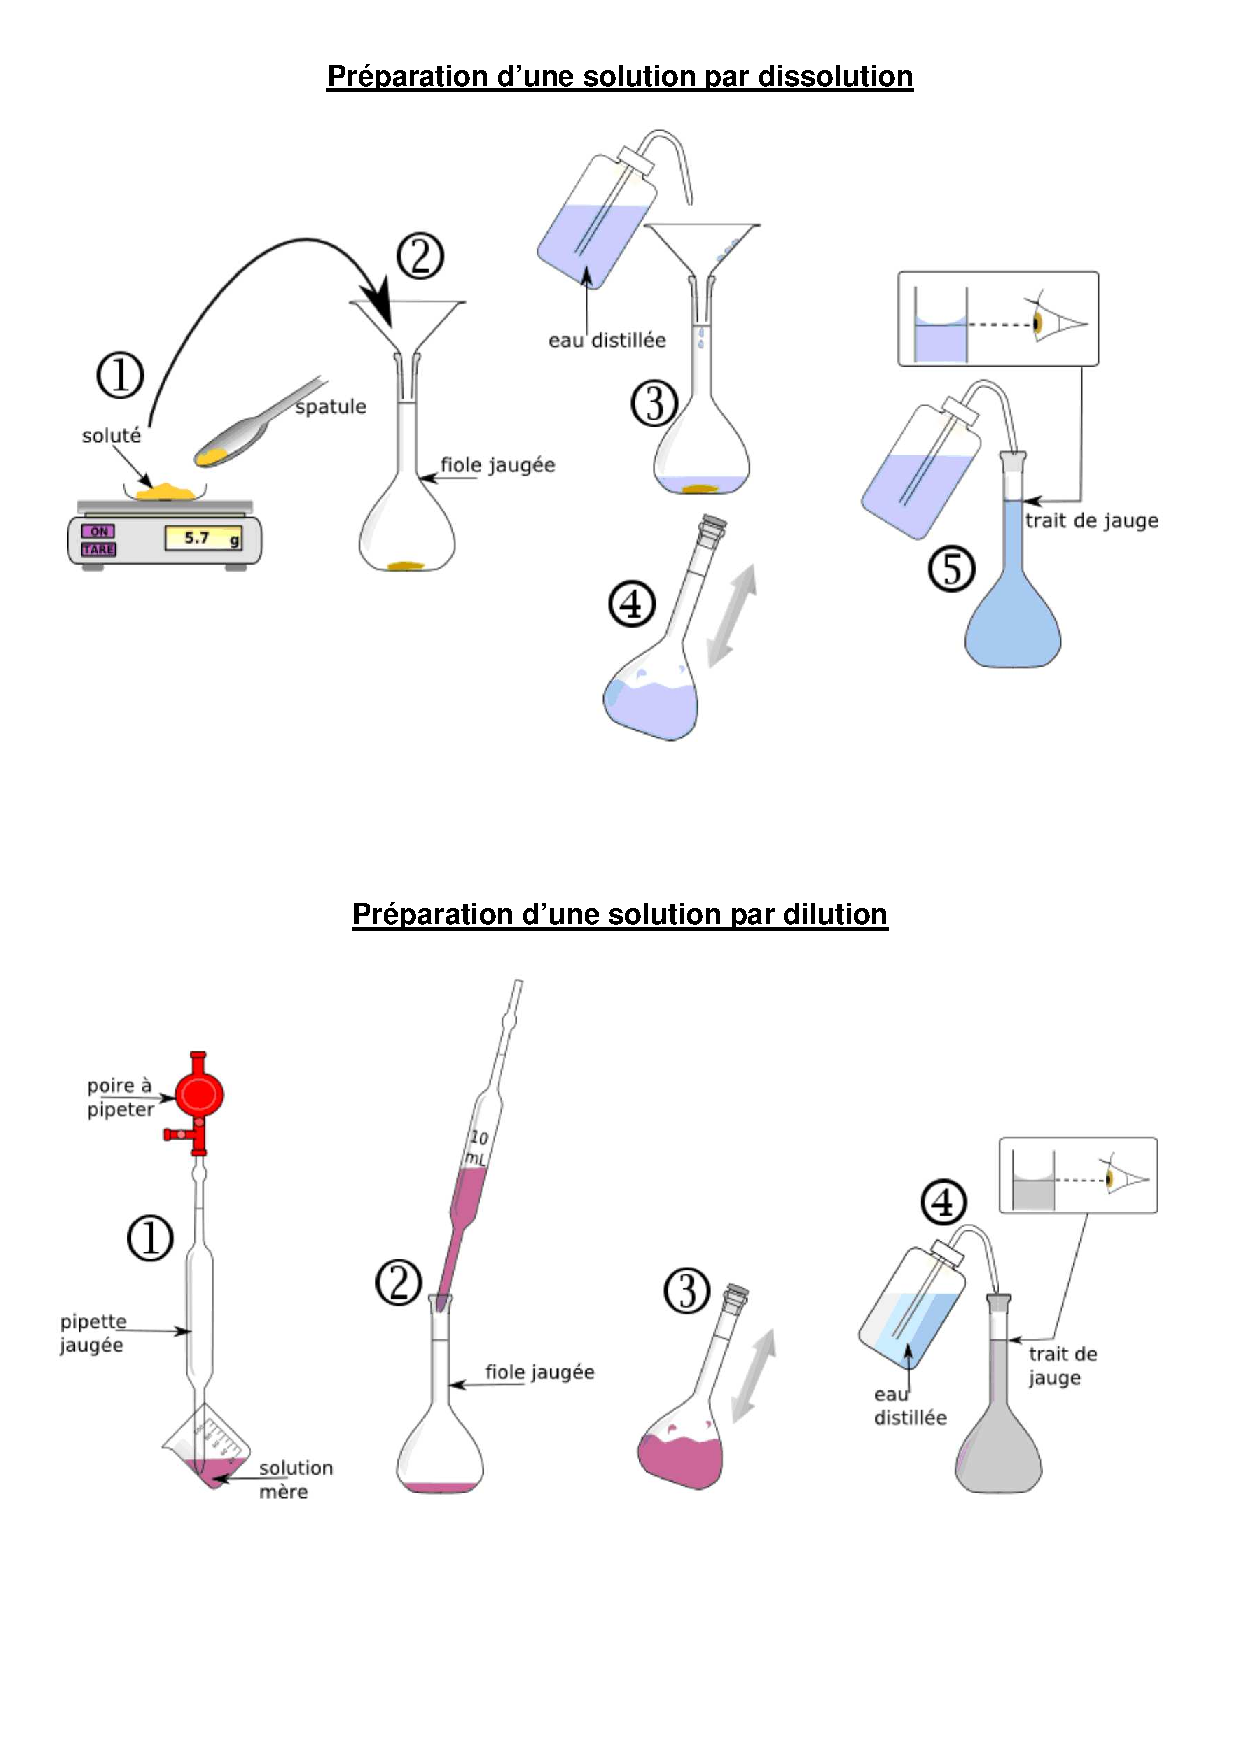
\includepdf[pages={-}]{dissolution_dilution}

\end{document}
